\section{Introduction}

Understanding the visual cortex and how patterns in images are interpreted in the brain has long been a goal of computational neuroscience. This article re-examines an early paper in the development of this field by Hancock et al. 1991 ~\cite{Hancock}. 
The aim of their paper is to use neural networks to perform Principal Component Analysis (PCA) on images. This technique finds a small set of linear descriptors that convey the most information about a set of images. The extremely high dimensional data from the images is projected onto a much smaller number of orthogonal axes which produce the most variation amongst the images. To do this exactly requires finding the eigenvectors of the correlation matrix of the input data. However this matrix is generally far too large to be done computationally. The paper applies neural network methods to solve this problem in a viable number of computations. An algorithm of Sanger's is used to produce receptive fields that converge to the principal components (PCs).\\
Hancock et al. showed that the receptive fields can detect features such as orientation in natural images and gaps between words in text images. The simplest of these receptive fields have also been found experimentally in the V1 cells of cats ~\cite{Orban}.

\section{Methods}

\subsection{Sanger's Algorithm}

Sanger's algorithm ~\cite{Sanger} creates a neural network where the principal components of input data are encoded into the strength of the network connections. Suppose we want to find the first $M$ PCs of $N$ dimensional input data. Then we create a network with $N$ input units and $M$ output units and define $w_{ij}$ to be the strength of the connection between the $i$th input unit and the $j$th output unit. For a sample of input data $\textbf{x}=(x_1,...,x_N)$ the output is defined to be:
\[y_j=\sum^N_{i=1}x_iw_{ij}\]
The connection strengths are then updated according to Sanger's rule:
\[\triangle w_{ij}=\eta y_j(x_i-\sum^j_{k=1}y_k w_{ik})\]
Here $\eta$ is the learning rate, chosen by the implementer. The algorithm is repeated with a new sample of input data $\textbf{x}=(x_1,...,x_N)$. For fixed $j$ the weight vector $w_{ij}$ can be shown to converge to the eigenvector of the correlation matrix of all the input data with $j$th largest eigenvalue ~\cite{Sanger}. This is the $j$th principal component of the data.

\subsection{Implementation to Images}

For each figure below a set of images was used as input data, given in Table \ref{tab:Table 1}. All images can be found in the re-implementation code. 
\begin{table}[h]
    \centering
    \begin{tabular}{ll}
    \hline
    Figures&Set of Images Used\\
    \hline
    1, 3, 4(a), 5&images1-15\\
    2, 4(b)&images1-15, new1-15, two0-9\\
    6, 7&textimage\\
    \hline
    \end{tabular}
    \caption{Images used in each figure.}
    \label{tab:Table 1}
\end{table}
Each of the images used was a 256x256 pixel greyscale image. Each pixel has a value from 0 to 255 corresponding to its grey level\\
64x64 pixel samples were taken by choosing a random image and a random area from it. The mean grey level was calculated from 20000 such samples. Sample input data was then prepared by taking a 64x64 pixel random sample, subtracting the mean grey level and then multiplying component wise by a Gaussian window of standard deviation 10 pixels centred at the centre of the image. This last step was done to reduce edge effects. The resulting 64x64 matrix was reshaped into a 1x4096 vector and normalised to unit length. This vector was then used as $\textbf{x}$ in Sanger's algorithm above.\\
Following the method of ~\cite{Hancock}, the network strengths $w_{ij}$ were initialised to random values between $\pm 0.03$. $\eta$ was initially set at 1 and reduced by a factor of a half every 20000 input samples for a total of 120000 samples.

\subsection{Description of Experiments}
Hancock et al. produce several sets of results studying different parts of their model which are reproduced below.
\subsubsection{Natural Image Experiments}
Firstly in their Figure 2 they extract the first 15 PCs from a run with 15 natural images. They display these as receptive fields - 64x64 pixel squares with grey level representing the strength of the connection to the input unit in that position. They repeat this using 40 natural images in their Figure 3 and note the similarity of the principal components.\\
Their next experiment is on orientation (Figure 4 in ~\cite{Hancock}). They aim to show that the orientation of the PCs is determined by the orientation of the images and not due to edge effects from the square samples. They complete a run with the original 15 images rotated by 45 degrees and extract the first 6 PCs, showing that they are indeed rotated as expected.\\
The variance experiment is given in Figure 5 in ~\cite{Hancock}. This aims to verify that the PCs are ordered by how much information they convey. They plot a log-log plot of the output variances of the first 15 PCs of the 15 image set (denoted by circles) and of the 40 image set (crosses). For each data point 10000 samples were used to calculate the output variance.\\
Next Hancock et al. investigate the effect of scale on the PCs of natural images. They repeat the run on the set of 15 natural images first at double the scale using 128x128 pixel sample sizes and a Gaussian window of size 20, and then at half the scale using 32x32 pixel sample sizes and a Gaussian window of size 5. The first 6 PCs are displayed in their Figure 6, and they note the lack of scale dependence.
\subsubsection{Text Image Experiments}
In Figure 7 in ~\cite{Hancock}, Hancock et al. repeat the scale experiment with text images, this time producing significant scale dependence. Four text images are used at three different magnification scales, with the first 8 PCs of each displayed. Scales which are proportional to the size of letters and line spacings are found in the PCs.\\
Finally, Hancock et al. show how the 7th PC of the finest scale images is tuned to gaps between words. They use the PC as a filter which they convolve with an original text image. Their Figure 8 shows that when this is thresholded and superimposed on the text images the word gaps are marked.

\subsection{Re-Implementation of Experiments}

Neither the original source code nor the original text images could be obtained, however the original natural images were obtained from the original authors. The model re-implementation was written in MATLAB using Sanger's algorithm and the presentation of images as described in the original paper.\\
For the rotation experiment, Hancock et al. rotate the natural images in a scanner and use the resulting images. Instead of doing this in the re-implementation, samples of the non-rotated images were chosen and then rotated using the MATLAB function "imrotate".\\
For the reproduction of the text image experiments a new text image was created by the author. This was done by copy-and-pasting text into a Word Document and editing it so it had similar features to the original text images. This included adding large whitespaces and finding a similar font. This was then converted into a PNG file and random sections of it at different scales were used as input to Sanger's algorithm to produce Figures 6 and 7 below. 

\subsection{Results}
All of the main features of Figures 2-8 in ~\cite{Hancock} were reproduced successfully. Results are given in Figures 1-7 below. Some images of PCs in the figures below are the negative images of those in the originals, but by the nature of Sanger's algorithm these represent the same PCs. Small differences were found in the order of the PCs, especially in the text image experiments, and the text image needed to be modified to produce a PC that detected word spacings.
 
\begin{figure}
    \centering
    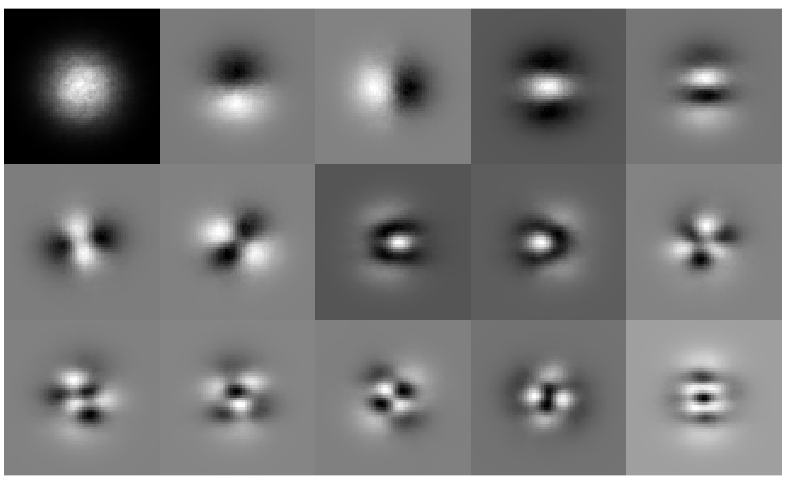
\includegraphics[scale=0.55]{figures/Figure1.png}
    \caption{Reproduction of the principal components of 15 natural images, numbered from top to bottom, left to right.}
    \label{fig:Figure1}
\end{figure}
\begin{figure}
    \centering
    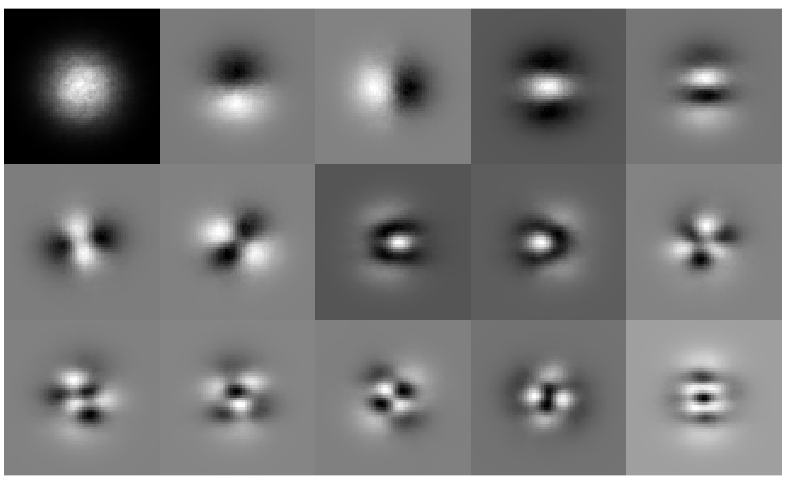
\includegraphics[scale=0.55]{figures/Figure2.png}
    \caption{The principal components of 40 natural images.}
    \label{fig:Figure2}
\end{figure}
\begin{figure}
    \centering
    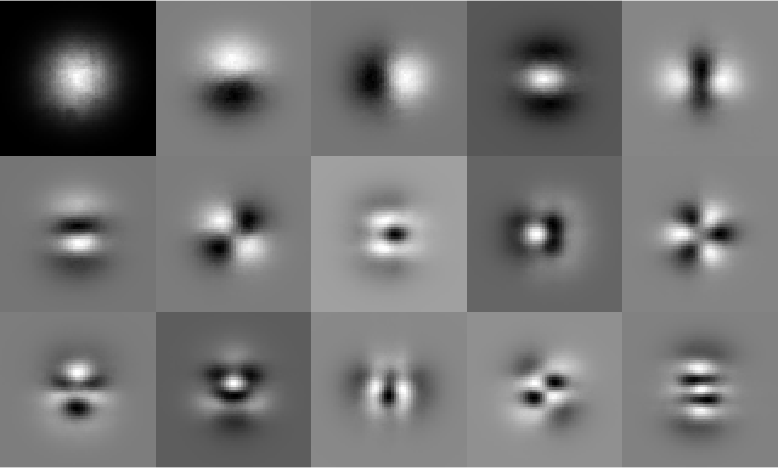
\includegraphics[scale=0.55]{figures/Figure3.png}
    \caption{Reproduction of the orientation experiment: the principal components of 15 natural images rotated by 45 degrees.}
    \label{fig:Figure3}
\end{figure}

\subsubsection{Natural Image Experiments}
The first 15 PCs of the set of 15 natural images are shown in Figure 1. These match those of ~\cite{Hancock}. The first component is approximately Gaussian. The second is the horizontal derivative of a Gaussian whilst the third is the vertical derivative. The relative ordering of the derivatives reflects the fact that horizontal correlation scales are longer than vertical scales in natural images.\\
Figure 2 repeats the first experiment with 40 natural images instead of 15. Again, the PCs match those found by Hancock et al. They are similar in features to those of the 15 natural images except with the ordering of some PCs swapped, namely 5 and 6, 10 and 11, and 13 and 14.\\
The rotation experiment is reproduced in Figure 3. PC numbers 5 and 6 are swapped in comparison with the original. The fact that the horizontal and vertical derivative operators are rotated by 45 degrees shows that the PCA is detecting the orientation of the images and not the edge effects of using a square sample. This matches the result found in ~\cite{Sanger}.\\
Figure 4 displays the reproduction of the variance experiment. The output variances of the PCs in Figure 1 and 2 were measured over 10000 samples of their respective input image sets. Figure 4 is a log-log plot of PC number against output variance. As found by ~\cite{Hancock}, the plot is approximately a straight line with variance decreasing with PC number. Hancock et al. found some minor deviations to this rule amongst PCs with very similar variance; the reproduction did not find this, instead finding that the PCs were ordered exactly by variance. This may have been down to the randomness of the inputs.\\
 The scale experiment on natural images is reproduced in Figure 5. The first 6 PCs at half the scale and at double the scale are displayed. These match those of ~\cite{Hancock} exactly apart from the ordering of the final two PCs at half the scale. They are also very similar to the PCs at the original scale, confirming the lack of scale dependence of correlations in natural images.\\
\begin{figure}
    \centering
    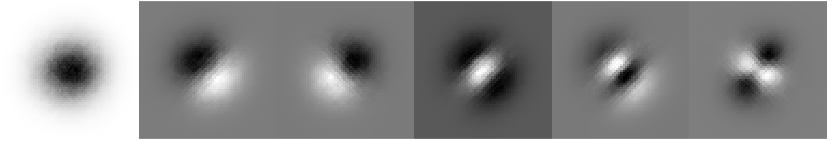
\includegraphics[scale=0.55]{figures/Figure4.png}
    \caption{Reproduction of the variance experiment: a log-log plot of output variance against PC number for (a) 15 natural images, (b) 40 natural images.}
    \label{fig:Figure4}
\end{figure}

 \begin{figure}
    \centering
    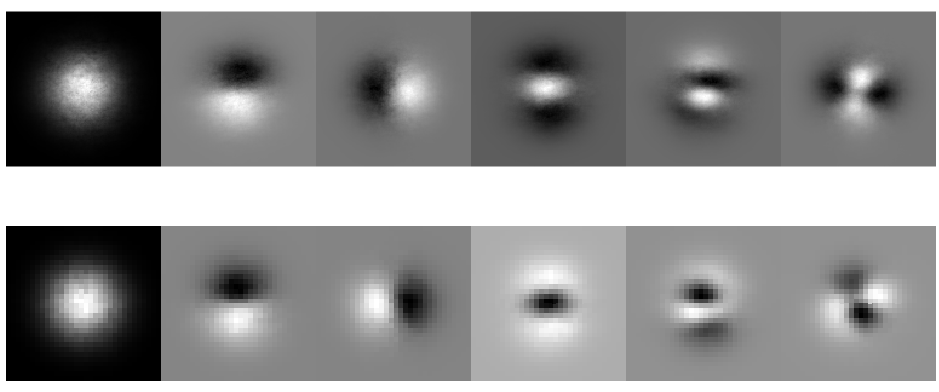
\includegraphics[scale=0.55]{figures/Figure5.png}
    \caption{Reproduction of the scale experiment for natural images: the principal components of 15 natural images at (a) double the scale, (b) half the scale.}
    \label{fig:Figure5}
\end{figure}

\subsubsection{Text Image Experiments}
The original text images could not be obtained, hence a new text image was prepared. It was in these experiments that the most difference was found with ~\cite{Hancock}.\\
The reproduced scale experiment on text images is found in Figure 6. The early PCs match those of Hancock et al. very well. The main finding that the PCs of text images depend on scale was reproduced: the first two PCs at each scale represent line size and the next two represent letter size. However the latter PCs were significantly different from ~\cite{Hancock}. In the finest scale the horizontal filters (PCs 3 and 4 in ~\cite{Hancock}) are missing from the reproduction, and the PC which marks word gaps is PC 5 rather than PC 7. This may have been due to the font used, as the shape and ordering of the PCs was found to be sensitive to font. Several fonts were used in initial trials of the reproduction, and displayed is the result of the most similar font the author could find to that used in ~\cite{Hancock}.\\
Figure 7 displays the convolution of the 5th PC at the finest scale with the full text image, which is then thresholded and superimposed over the text image. As found in ~\cite{Hancock}, this marks gaps between words. For this to be reproduced, further experimental modifications had to be made to the text image. Text with no large whitespace or font that was too thin failed to produce a PC that corresponded to word spacings. As mentioned above, when such a PC could be produced it was the 5th PC not the 7th as in ~\cite{Hancock}. 
\begin{figure}
    \centering
    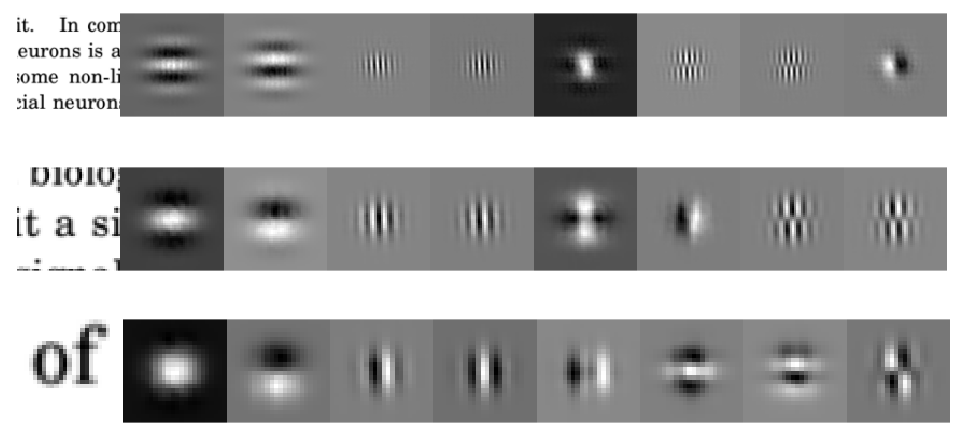
\includegraphics[scale=0.55]{figures/Figure6.png}
    \caption{Reproduction of the scale experiment for text images: samples of text and their principal components at (a) double, (b) original, (c) half scale.}
    \label{fig:Figure6}
\end{figure}
\begin{figure}
    \centering
    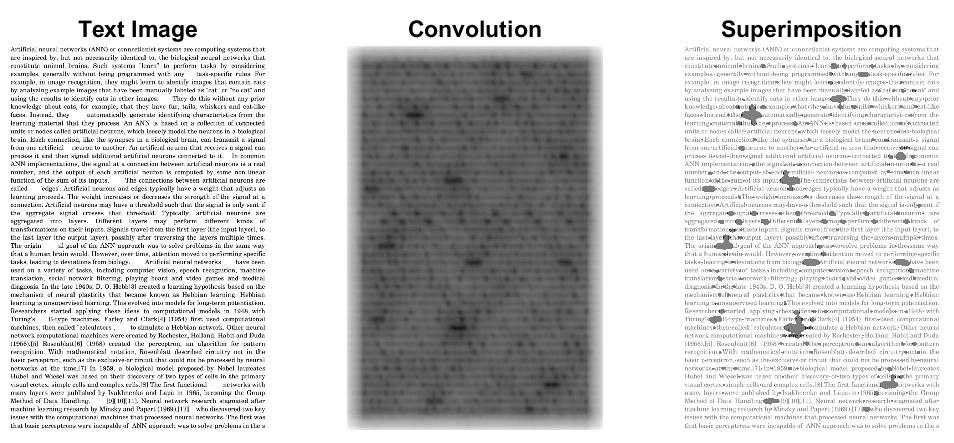
\includegraphics[scale=0.55]{figures/Figure7.png}
    \caption{Reproduction of the convolution experiment: (a) The full text image. (b) The text image convolved with PC 5 from Figure 6(a). (c) The convolution thresholded and superimposed over the text image.}
    \label{fig:Figure7}
\end{figure}

\section{Conclusion}
Our re-implementation of Principal Component Analysis using Sanger's algorithm from Hancock et al. 1991 was successful in reproducing the main results and most principal components from the original paper. The main results concerning orientation dependence (Figure 3), variance (Figure 4) and scale dependence (Figures 5 and 6) in ~\cite{Hancock} are reproduced well. The primary principal components are reproduced in all experiments and although there are differences in the latter principal components of text images, the re-implementation was able to extract a PC that marked word gaps (Figure 7).\\
The description of the model in the original paper was clear and was sufficient to write a re-implementation without the source code. All model parameters are stated clearly and the method of preparing the input image samples was simple to follow. Obtaining the original natural images also allowed for results to be reproduced easily and faithfully. The main difficulty in reproduction was the creation of a new text image that recreated the desired principal components. This required some trial and error as the principal components are sensitive to font and features in the text suggesting that some of the results in ~\cite{Hancock} are particular to the images used.